\section{Architektur}

\paragraph{Grundmodell}
\begin{itemize}
	\item Daten überbrücken räumliche Distanz (abstrakten Übertragungsabschnitt)
	\item Abstraktion auf Basis von \textbf{Schichten}, stellen Dienste über Schnittstellen bereit
	\item Höhere Schicht erfordert Dienste der darunterliegenden Schicht
	\item \textbf{Ziele}:
	\begin{itemize}
    \item Komplexitätsreduktion (Vereinheitlichung, Modularisierung)
    \item Interoperabilität (Hersteller-/Systemunabhängigkeit)
    \item Flexibilität und Erweiterbarkeit
  \end{itemize}
	\item \textbf{Horizontale Kommunikation}: zwischen Sender und Empfänger, Protokollinstanzen einer Schicht tauschen Daten aus um Dienst zu erbringen
	\item \textbf{Vertikale Kommunikation}: zwischen verschiedenen Schichten in einem System, Protokollinstanz Schicht n greift auf Dienste von Protokollinstanz Schicht n-1 zu
\end{itemize}

\paragraph{OSI-Referenzmodell}
\begin{itemize}
\item \textbf{Logisches} Modell, nicht Implementierungsmodell
\item Keine Protokolle (nur Prinzipien), offener Standard
\item Unterteilung in Transportsystem (1-4) und Anwendungssystem (5-7)
  \item \textbf{Schicht 1}: Bit-Übertragungsschicht (\emph{physical layer})
  \begin{itemize}
    \item \emph{Ziel}: Übertragungsqualität
    \item Bitübertragung
    \item Verwendung von Leitungscodes usw
    \item \emph{keine} Pufferung, \emph{kein} zuverlässiger Dienst
  \end{itemize}
  \item \textbf{Schicht 2}: Sicherungsschicht (\emph{data link layer})
  \begin{itemize}
    \item \emph{Ziel}: Kommunikation zwischen physikalisch benachbarten Systemen
    \item Erkennung/Behebung von Fehlern der Bitübertragungsschicht
    \item Bitstrom in Rahmen gliedern
    \item Puffern bei Sender + Empfänger
  \end{itemize}
  \item \textbf{Schicht 3}: Vermittlungsschicht (\emph{network layer})
  \begin{itemize}
    \item \emph{Ziel}: Verknüpfung von Übertragungsabschnitten zu Netz
    \item Wegewahl im Kommunikationssystem
    \item Geräteadressierung, Multiplexing
  \end{itemize}
  \item \textbf{Schicht 4}: Transportschicht (\emph{transport layer})
  \begin{itemize}
    \item \emph{Ziel}: Übertragung von Daten zwischen Anwendungen
    \item Abstrahiert von Diensten der Vermittlungsschicht
    \item Fehlererkennung/-behebung
    \item Pufferung, Multiplexing
    \item Adressierung von Transportdienstnutzern
  \end{itemize}
  \item \textbf{Schicht 5}: Sitzungsschicht (\emph{session layer})
  \begin{itemize}
    \item \emph{Ziel}: Nichtunterbrechbarkeit von Kommunikationsbeziehungen
    \item Datenaustausch-Gliederung nach Gesichtspunkten der Anwendung
    \item Ablaufsteuerung/Koordination
    \item Bereitstellen von Sitzungen
  \end{itemize}
  \item \textbf{Schicht 6}: Darstellungsschicht (\emph{presentation layer})
  \begin{itemize}
    \item \emph{Ziel}: Einheitliche Datendarstellung
    \item Kommunikation zwischen heterogenen Geräten
    \item Beibehaltung der Informationssemantik bei Überführung der Syntax
  \end{itemize}
  \item \textbf{Schicht 7}: Anwendungsschicht (\emph{application layer})
  \begin{itemize}
    \item \emph{Ziel}: Austausch anwendungsabhängiger Daten
  \end{itemize}
\end{itemize}

\paragraph{Internet-Referenzmodell}
\begin{itemize}
  \item Einfacheres Modell, nur 4 Schichten (manchmal 5 bei Trennung von Sicherung und Bit-Übertragung)
  \item Darstellungs- und Sitzungsaufgaben in Anwendungen verlagert
\end{itemize}

\paragraph{Datenkapselung}
\begin{itemize}
	\item Information wird durch alle Schichten durchgereicht
	\item Daten werden in jeder Schicht gekapselt (mit Header und/oder Trailer versehen)
\end{itemize}
\begin{figure}[H]\centering\label{KapselungInternet}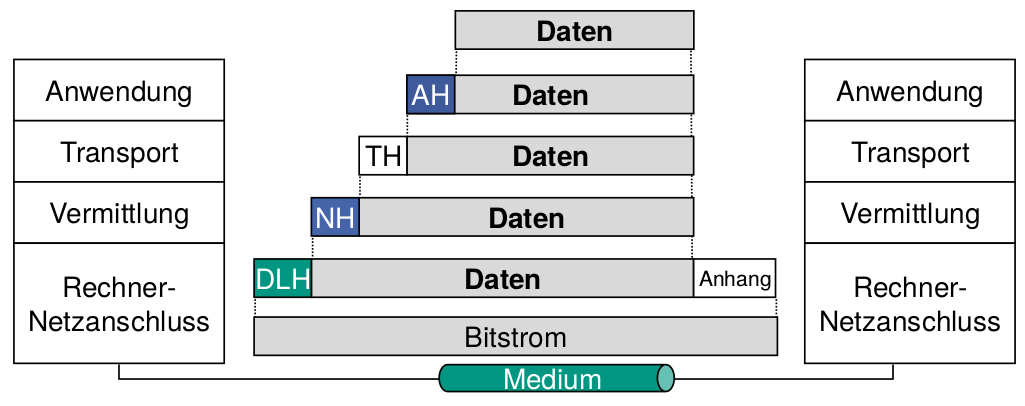
\includegraphics[width=.7\linewidth]{KapselungInternet}\end{figure}

\paragraph{Protokolle}
Regeln und Formate für Datenaustausch \emph{innerhalb} einer Schicht

\paragraph{Dienste}
\begin{itemize}
  \item Bündelung zusammengehöriger Funktionen
  \item Zusammenwirkung von Protokollinstanzen \emph{innerhalb} einer Schicht
  \item Schichten gehen über gesamtes Kommunikationssystem hinweg
  \item \emph{Dienstfunktion}: einzelne Dienstteile unabhängig voneinander nutzbar
  \item \emph{Dienstprimitiv}: Einzelvorgänge einer Dienstfunktion
  \begin{itemize}
    \item \emph{request} (Req): Beauftragung (Nehmer \( \to \) Geber)
    \item \emph{indication} (Ind): Partnerbenachrichtigung (Nehmer \( \leftarrow \) Geber)
    \item \emph{response} (Rsp): Partnerbeantwortung (Nehmer \( \to \) Geber)
    \item \emph{confirmation} (Cnf): Abschlussbenachrichtigung (Nehmer \( \leftarrow  \) Geber)
  \end{itemize}
  \item \emph{Dienstehierarchie}: Dienst baut auf anderen Diensten auf \\* (Dienstbringer/-nehmer)
  \item \emph{Dienstzugangspunkte}: Dienstschnittstellen
\end{itemize}

\paragraph{Ablauf --- Webseitenaufruf}
\begin{itemize}
  \item \textbf{Start}: Einstecken Netzwerkkabel
  \item \textbf{Ende}: Seitenempfang
  \item \textbf{Netzverbindung}: IP erhalten, Router + DNS kennenlernen
  \begin{enumerate}
    \item DHCP-Anfrage (verpackt in UDP, IP, 802.3)
    \item Ethernet-Paket wird im LAN gebroadcastet
    \item DHCP-Server im Router empfängt + entpackt Paket
    \item DHCP-Server erstellt DHCP ACK-Paket mit Client-IP, Router-IP, DNS-IP
    \item DHCP-Antwort wird verpackt und direkt an Client gesendet
    \item Client empfängt und entpackt Paket
  \end{enumerate}
  \item \textbf{ARP}: MAC des Routers kennenlernen
  \begin{enumerate}
    \item ARP-Anfrage an Broadcast-Adresse
    \item Router sendet seine MAC in ARP-Antwort
  \end{enumerate}
  \item \textbf{DNS}: IP-Adresse der angeforderten Webseite kennenlernen
  \begin{enumerate}
    \item IP-Datagramm mit DNS-Anfrage wird von LAN-Switch zu lokalem Router geleitet
    \item IP-Datagramm: lokales Netz \( \to \) ISP-Netz \( \to \) DNS-Server (mit RIP oder OSPF)
    \item Paket wird an DNS-Server entpackt
    \item DNS-Server antwortet Client mit angeforderter IP
  \end{enumerate}
  \item \textbf{TCP}: Aufbau einer TCP-Verbindung
  \begin{enumerate}
    \item Eröffnung eines TCP-Sockets zum Webserver
    \item TCP-SYN-Segment wird zu Server geroutet
    \item Server antwortet mit SYNACK
  \end{enumerate}
  \item \textbf{HTTP}: Webseite laden
  \begin{enumerate}
    \item HTTP-Anfrage wird per TCP-Socket gesendet
    \item IP-Datagramm mit HTTP-Anfrage wird zu Webserver geroutet
    \item Server antwortet mit HTTP-Antwort
    \item IP-Datagramm mit HTTP-Antwortet wird zurück zu Client geroutet
  \end{enumerate}
\end{itemize}